\section{Results}
\label{sec:m4lresults}
This section presents the results of the inclusive four-lepton analysis published in Reference \cite{m4l2021_paper} by the \ATLAS collaboration. The measured fiducial cross-sections are presented in Table~\ref{tab:fidxs}. The first column shows the cross-section measured in the full fiducial phase space, while the subsequent columns quote the cross-section in the four \mFourL{} regions dominated by \ZFourL{}, \HFourL{}, \onshellZZ{}, or \offshellZZ{} production. The theoretical predictions for the cross-sections in these regions are also provided in the bottom two rows. The two predictions differ in the choice of generator used to simulate the dominant \qqFourL{} process; one uses \SHERPA at NLO accuracy in QCD and the other uses \POWHEG interfaced to \pythia{} normalized to a NNLO prediction. Details of the theoretical predictions can be found in Section~\ref{sec:montecarlopred}.

The associated uncertainties are also presented. For the measured cross-sections, the total combined uncertainty as well as the uncertainties split into three categories (statistical, systematic, or luminosity) are given. For more on the uncertainty breakdown and how they are estimated, see Section \ref{sec:uncertainties}. The data are slightly higher than both predictions in all but the \ZFourL{} region, where it lies between the \SHERPA{} and \POWHEG{} + \pythia{} predicted values. In general, the \SHERPA{} predictions are higher than the \POWHEG{} + \pythia{} predictions, with the \onshellZZ{} region being an exception. Overall, the measured data are in good agreement with both predictions within the quoted uncertainties. The largest differences comes from the \onshellZZ{} region where the data is around one sigma higher than the predicted \SHERPA{} value. 

% In Ref.~\cite{ATLAS:2020wny} the \HFourL{}  cross-section is measured
% by ATLAS in a fiducial phase space that differs slightly from the \HFourL{} region measured here. The phase space is designed to minimise the contribution from non-\HFourL{} processes. In the dedicated Higgs measurement the cross-section is found to be slightly below the SM prediction. The dedicated Higgs measurement differs from the present measurement in using a slightly different phase space, in subtracting
% non-Higgs processes using a data-driven approach, and in including a $\sim1\%$ contribution from  Higgs production in association with a $b$-quark pair in the prediction.
\begin{table}[t] 
  \centering
    \begin{tabular} {c c c c c c }
      \hline
      & \multicolumn{5}{c}{Region} \\
      & Full   & $Z\rightarrow 4\ell$  & \HFourL{}  & Off-shell $ZZ$  & On-shell $ZZ$   \\
      \hline
      Measured        & 88.9              & 22.1              & 4.76                & 12.4                & 49.3 \\
      fiducial & $\pm$1.1 (stat.\,)    & $\pm$0.7 (stat.\,)    &  $\pm$0.29 (stat.\,)  & $\pm$0.5 (stat.\,)     & $\pm$0.8 (stat.\,) \\
      XS $[$fb$]$     & $\pm$2.3 (syst.\,)    & $\pm$1.1 (syst.\,)    &   $\pm$0.18 (syst.\,) & $\pm$0.6 (syst.\,)     & $\pm$0.8 (syst.\,) \\
       			         & $\pm$1.5 (lumi.)    & $\pm$0.4  (lumi.)  & $\pm$0.08 (lumi.)	   & $\pm$0.2 (lumi.)	   &   $\pm$0.8 (lumi.) \\
                              & $\pm$3.0 (total\,)   & $\pm$1.3 (total\,)   &   $\pm$0.35  (total\,)   & $\pm$0.8 (total\,)    &   $\pm$1.3 (total\,) \\
      \hline
      \SHERPA{}                            & 86$\pm$5          & 23.6$\pm$1.5      & 4.57$\pm$0.21       & 11.5$\pm$0.7       & 46.0$\pm$2.9 \\
      \POWHEG         & 83$\pm$5          & 21.2$\pm$1.3      & 4.38$\pm$0.20       & 10.7$\pm$0.7       & 46.4$\pm$3.0 \\
      + \pythia{} & & & & & \\
      \hline
   \end{tabular}
   \caption{Fiducial cross-sections in the full fiducial phase space and in the \ZFourL{}, \HFourL{}, \onshellZZ{}, and \offshellZZ{} dominated regions in femtobarns. They are compared with two particle-level predictions and their uncertainties where the \qqFourL{} process is simulated with either \SHERPA{} or with \POWHEG{} + \pythia{}. \label{tab:fidxs} }
\end{table}
Figure \ref{fig:cross-sec-m4l} presents the differential cross-section as a function of \mFourL{}, as well as two predicted SM cross-sections
where either \SHERPA{} or \POWHEG{} is used to model the \qqFourL{} contribution. The breakdown of the SM processes in the predictions are plotted in colour and stacked. Various features corresponding the different physics processes are visible in this plot. At \mFourL{}=$m_\Z\simeq 91.19$~GeV~\cite{pdg_2021} there is the single resonant \Z peak, and similarly for the \mFourL{}=$m_{H}\simeq125.10$~\cite{pdg_2021} for the Higgs. An enhancement is visible at \mFourL{}=$2m_\Z\simeq 182$~GeV when the on-shell production of two \Z bosons becomes possible. Overall, the SM predictions are in agreement with the measurement within the quoted uncertainties for the entire distribution.
\todo[inline]{Discuss the dominant stat uncertainty, and other uncertainty sources.}

A $p$-value quantifies the probability of finding the data at least as extreme as the data observed \cite{cowan_munich}, with $n$ degrees of freedom equal to the number of bins. There are two $p$-values shown (one for each SM prediction using either \SHERPA{} or \POWHEG{} to model \qqFourL{}) for the inclusive \mFourL{} of Figure \ref{fig:cross-sec-m4l} and all other distributions. The $p$-value is derived from the $\chi^2$, which is defined as:
\begin{equation}
    \chi^2 = \left[ \sigdata - \sigpred \right] ^T C^{-1} \left[  \sigdata - \sigpred  \right]
\end{equation}
where \sigdata{} and \sigpred are $n$-dimensional vectors representing the binned measured and predicted differential cross-sections, and $C$ is the $n\times n$ summed total covariance matrix which accounts for the combination of statistical and systematic uncertainties. For the inclusive \mFourL{} distribution, the calculated $p$-value for the data is $p=0.22$ for the \SHERPA{} prediction and $p=0.09$ for the \POWHEG{} prediction, echoing the results in Table \ref{tab:fidxs} where the \SHERPA{} prediction is the higher of the two and the data are higher than both predictions. 
\begin{figure}[h]
  \centering
  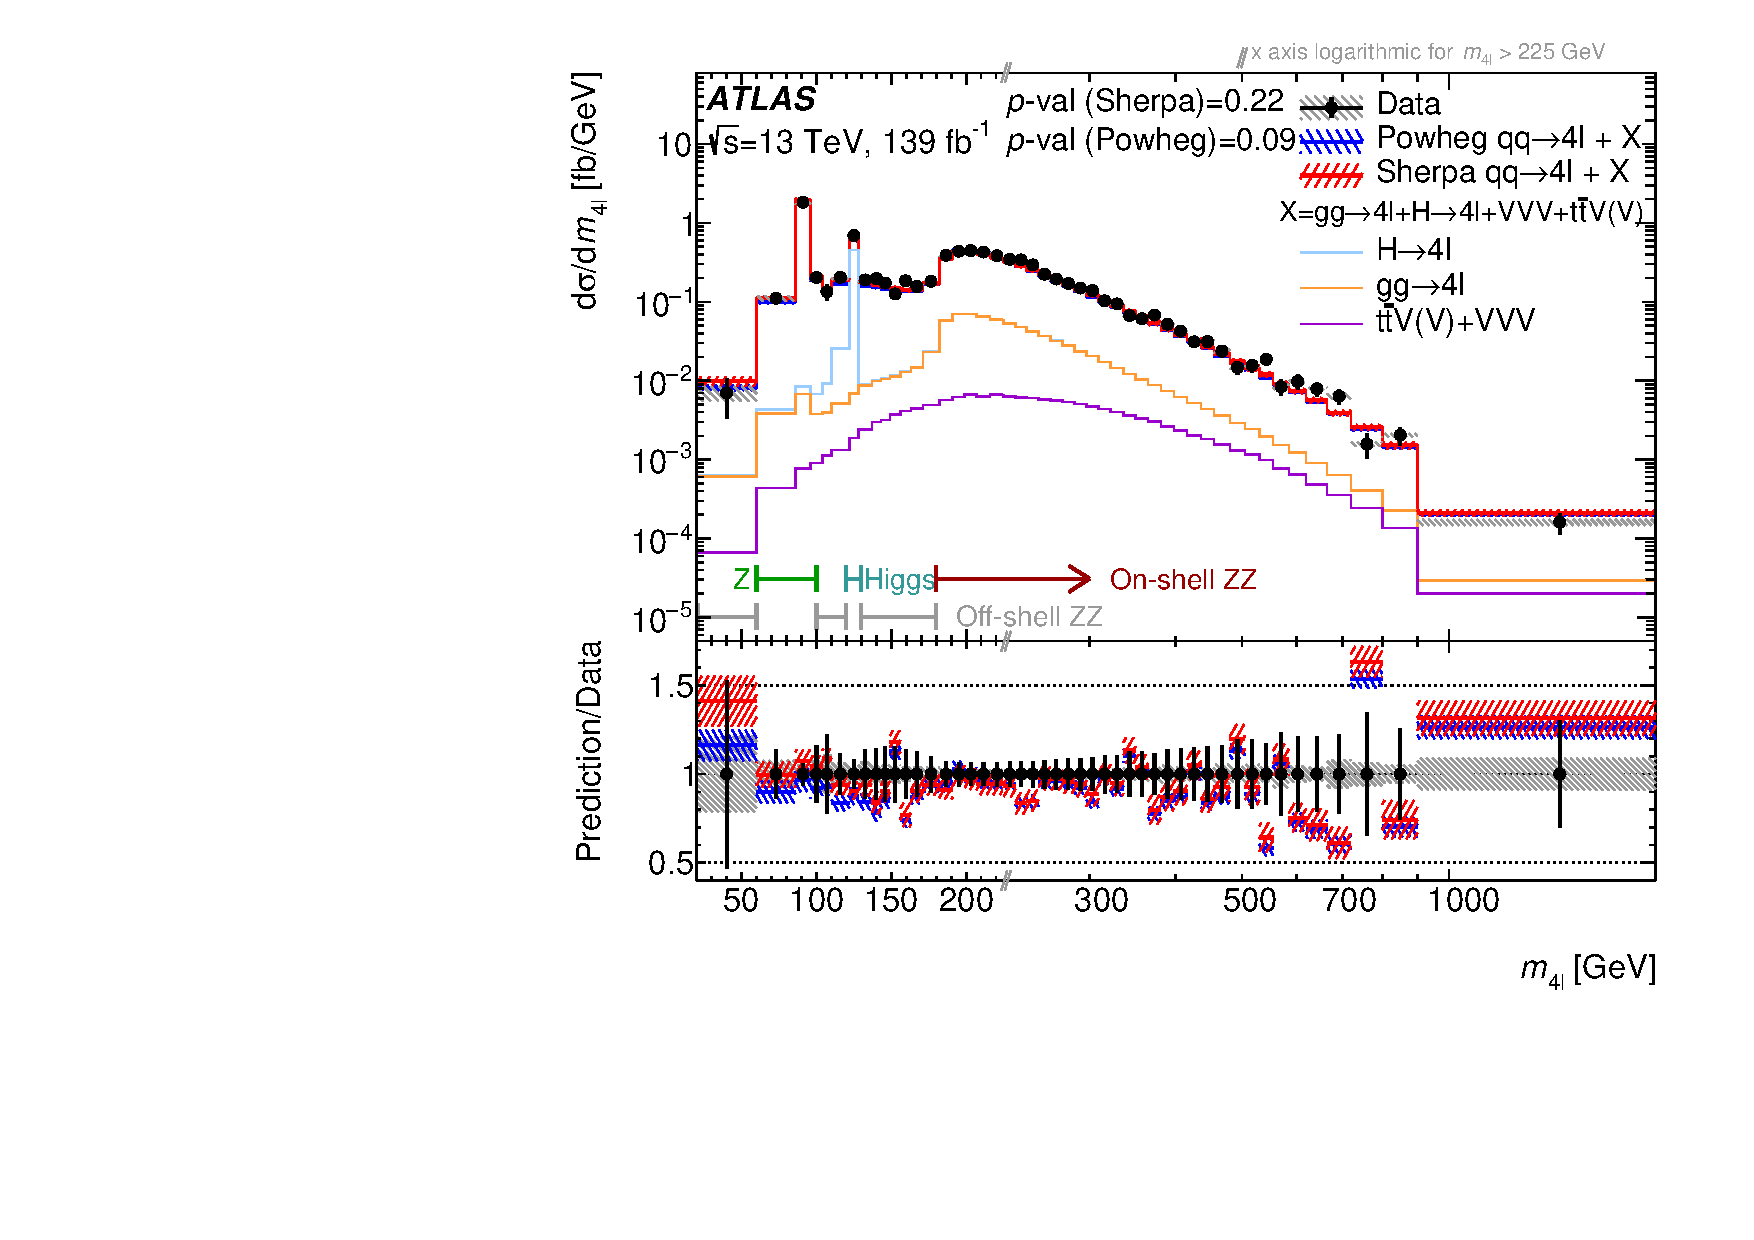
\includegraphics[width = 0.7\textwidth]{Figures/m4l/UnfoldedResults/linlog_Unfolded_Data_inclm4l.pdf} 
    \caption{Differential cross-section as a function of the four-lepton invariant mass \mFourL as measured in data in black. \errorbars{} \SMpredictions{} 
    The coloured stacked histograms represent the per-process breakdown of the SM prediction. In the lower left corner of the figure, boundary lines are drawn to indicate the four different \mFourL{} regions, each dominated by a different process. \Pvalue{} 
    The ratio of the \SHERPA{} and \POWHEG{} prediction to the data is shown in the lower panel. The $x$-axis is on a linear scale until $\mFourL = 216$~\GeV, where it switches to a logarithmic scale. \label{fig:cross-sec-m4l}}
\end{figure}

Figure \ref{fig:m4l_pt4l} shows the differential cross-section as a function of \mFourL{} in five slices of the four-lepton transverse momentum, \ptFourL{}. Likewise in Figure \ref{fig:m4l_y4l} the \mFourL{} spectrum is plotted in five slices of $|\yFourL{}|$, the absolute rapidity of the four-lepton system. Figure \ref{fig:m4l_flavour} contains three subplots of the differential cross-section as a function of \mFourL{} in the $4e, 4\mu$ and $2e2\mu$ flavour channels. There is good agreement between the data and the SM predictions overall for these distributions, however, the \POWHEG{}+\pythia{} prediction in the $100 < \ptFourL{} < 600~\GeV$ slice and the $0.9 < \yFourL{} < 1.2$ slice are below the data, resulting in low $p$-values ($p = 0.008$ and $p = 0.003$ respectively). These features reflect the results presented in Table~\ref{tab:fidxs}. The third mass bin of Figure~\ref{fig:m4l_pt4l} (b) displays a large discrepancy between data and prediction, where both the \SHERPA{} and \POWHEG{} prediction are over two times larger. This feature is also present in the reconstruction level results, and therefore is not a by product of the unfolding process.

The cross-section as a function of the dilepton mass of the primary and the secondary lepton pair, \mZOne{} and \mZTwo{}, are presented in Figures \ref{fig:m12_m4l} and \ref{fig:m34_m4l} in the different \mFourL{} regions. In the region dominated by Higgs production, the Higgs contribution is drawn separately in blue. For \mZOne{}, a peak is visible at $m_{\Z}$ in all but the \ZFourL{} region. \mZTwo{} on the other hand has the $m_{\Z}$ enhancement only in the \onshellZZ{} region where it is kinematically allowed. The \ZFourL{} and \offshellZZ{} regions of \mZTwo{} are dominated by off-shell \Z boson and photon exchange, while the \HFourL{} region is dominated by off-shell \Z production. In the third mass bin of the Higgs slice of \mZTwo{} shown in Figure~\ref{fig:mZ2unf}, the theoretical predictions are more than two times higher than the observed data. Once again, this feature is also present in the reconstruction level results. There are some low $p$-values for these observables, notably in the \onshellZZ{} region of \mZOne{}, and the \HFourL{} and \offshellZZ{} region of \mZTwo{}. These are attributed to features discussed in Table \ref{tab:fidxs}, paired with statistical fluctuations in the data and differences in modelling between the two generators. 

The transverse momentum of the leading and sub-leading lepton pair in the four \mFourL{} regions are presented in Figures \ref{fig:pt12_m4l} and \ref{fig:pt34_m4l}. In the \onshellZZ{} region for both the spectrum peaks at around \unit{40}{\GeV}. For the other three regions, the peak is approximately \unit{20}{\GeV}. The shapes of all slices for both \ptZOne{} and \ptZTwo{} are similar, with a steady rise to the peak and a slow fall into the high $p_T$ tail. There is a notable disagreement between observation and prediction in \ptZTwo{}. An under-prediction of the cross-section for low \pT in \onshellZZ{} region is visible. This was already observed in prior ATLAS measurements of $ZZ$ diboson production~\cite{Aaboud:97.032005}.

The variables \CTSOneTwo{} and \CTSThreeFour{} are sensitive to the polarization of the decaying bosons, and can serve as a probe for new physics \cite{Denner_2020}. For each lepton pair, $\theta^*$ is defined as the angle between the negative lepton in the \Z rest frame and the \Z boson in the lab frame. Figures \ref{fig:cts12_m4l} and \ref{fig:cts34_m4l} show the polarization variables leading and sub-leading lepton pair, \CTSOneTwo{} and \CTSThreeFour{}, in the \mFourL{} regions. There is good agreement between data and prediction for all distributions. 

The unfolded cross-section in the \mFourL{} regions for the azimuthal angle between the leading and sub-leading leptons of the quadruplet, \dPhill{}, is shown in Figure \ref{fig:dPhill_m4l}. Studied in detail in Reference \cite{Gutschow_2021}, this variable is sensitive to next-to-leading order electroweak corrections on four lepton production. The shape of the distributions in the four regions are largely similar, peaking at \dPhill{}$\approx\pi$ when the leading and sub-leading leptons are in opposite hemispheres. Good agreement with the SM prediction is seen throughout.

Figures \ref{fig:dPhiPairs_m4l} and \ref{fig:dYPairs_m4l} show the azimuthal angle difference and the rapidity difference between the lepton pairs. In the \offshellZZ{} and \onshellZZ{} region of \dPhiPairs{}, the low $p$-values are mainly driven by statistical fluctuations in the data alongside low SM predictions for \dPhiPairs{}$<\frac{26}{64}\pi$. The \dYPairs{} distributions peak at zero and with a gradual tail to five. In the \onshellZZ{} region of \dYPairs{}, the SM prediction drops to be up to 50\% lower than the data at high values, indicating mis-modelling by the MC generators. 

